\clearpage
\section{Umsetzung Benchmark}\label{sec:ZigbeeUmsetzungBenchmark}
\todo[inline]{Komplette Beschreibung der Firmware unterteilt in die 3 Nodetypen. Besonderheiten herausstreichen und allfällige Schwierigkeiten aufzeigen.}

Die Umsetzung des Benchmarks geschah im Rahmen der Anforderungen des Benchmark Konzepts gemäss Abschnitt \ref{sec:BenchmarkKonzeptMeshNetzwerke}.
Wie im Abschnitt \ref{sec:Soft-undFirmware} bereits ausführlich behandelt, sind innerhalb der Shared Library (siehe Abschnitt \ref{subsec:SharedLibrary}) klare Schnittstellen und Grenzen für die Mesh Protokollstacks definiert.
Nachfolgend wird auf die Umsetzung des Zigbee Stacks innerhalb dieser Grenzen eingegangen.

\subsection{Zigbee Software Development Kit}\label{subsec:ZigbeeSoftwareDevelopmentKit}
Für die Umsetzung von Zigbee Applikationen auf dem nRF52840 SoC \ref{subsec:SystemonChip} stellt Nordic Semiconductor ein eigenes Software Development Kit (SDK) zur Verfügung, die \textit{nRF5 SDK for Thread and Zigbee} \cite{nordic_semi_nrf_sdk_for_thread_and_zigbee_2020}.
Da Thread und Zigbee den selben \textit{IEEE 802.15.4} MAC Layer benutzen, teilen sich die beiden Protokollstacks eine gemeinsame SDK.
Innerhalb der SDK nutzen die beiden jedoch unterschiedliche Ressourcen.

\begin{figure}[h]
	\centering
	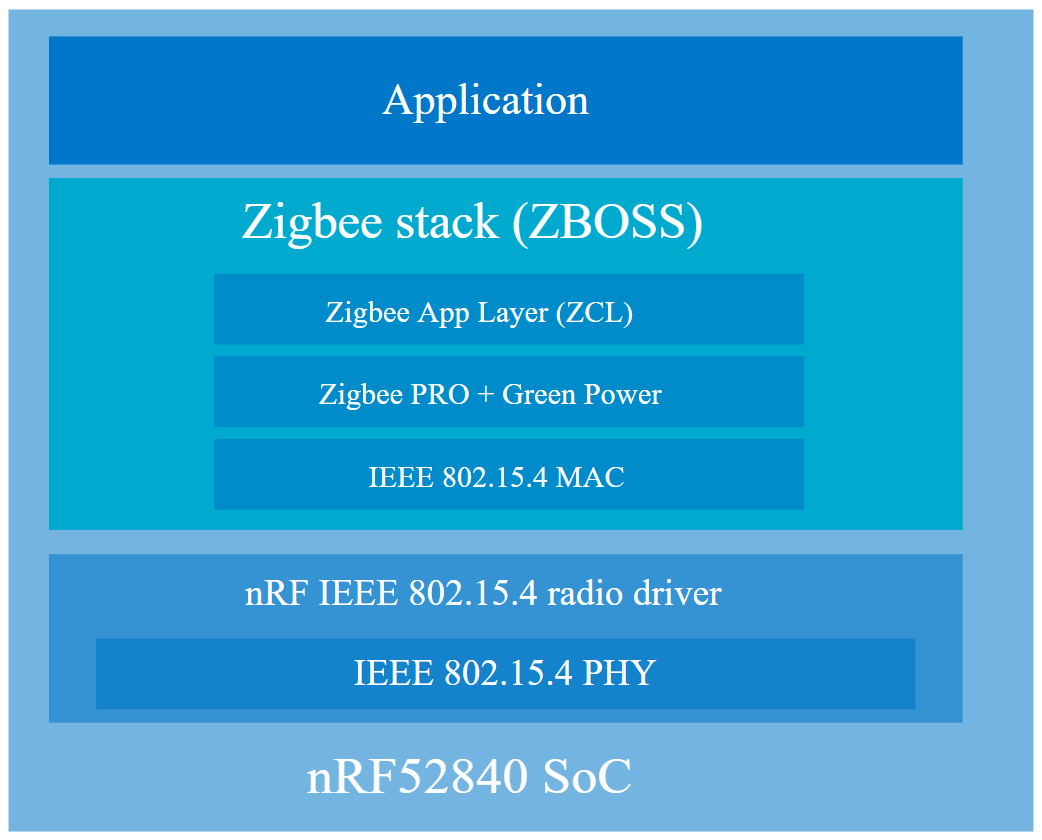
\includegraphics[width=0.6\textwidth]{Zigbee_SDK_Plattform_Design.png}
	\caption{nRF5 SDK for Thread and Zigbee Plattform Design Referenz für Zigbee Applikationen \cite{nordic_semi_nrf_sdk_for_thread_and_zigbee_2020}}
	\label{fig:ZigbeePlattformDesign}
\end{figure}

Für Zigbee Applikationen kommt ein Plattform Design gemäss Abbildung \ref{fig:ZigbeePlattformDesign} zum Einsatz. 
Als eigentlicher Zigbee Stack wird der \textit{ZBOSS} Zigbee Stack in der Version 3.3 von DSR\footnote{ZBOSS stack v3.3.0: \url{https://dsr-iot.com/}} implementiert.
Es handelt sich dabei um einen weit verbreiteten \textit{Zigbee PRO} Stack welcher die neuste Version der Zigbee Core Specification rev22 umsetzt.
\textit{ZBOSS} verwendet dabei ein kooperatives Multitasking Prinzip mit einem Scheduler welche die Tasks verwaltet.

Unter dem \textit{ZBOSS} Stack verwendet die SDK den \textit{nRF IEEE 802.15.4 radio driver} für die Ansteuerung der Funkschnittstelle.
Über dem \textit{ZBOSS} Stack befindet sich die Applikationsebene in welcher Applikationen gemäss den ZCL Spezifikationen\footnote{\url{https://zigbeealliance.org/wp-content/uploads/2019/12/07-5123-06-zigbee-cluster-library-specification.pdf}\cite{the_zigbee_alliance_zigbee_2016}} umgesetzt werden können.
\textit{ZBOSS} stellt die dafür notwendigen Funktionen zur Verfügung.


\subsection{Zigbee Stack Implementation}\label{subsec:ZigbeeStackImplementation}
Der Zigbee Stack wurde mit Hilfe der \textit{nRF5 SDK for Thread and Zigbee} wie oben beschrieben implementiert.
Dabei wurden einige Funktionen und Werte definiert.
Diese sollen in den nächsten Abschnitten erläutert werden.

\subsubsection{Topologie}\label{subsubsec:ZigbeeTopologie}
Das Zigbee Netzwerk für den Benchmark wurde mit Hilfe des \textit{ZigBee PRO} Stackprofils als vollständiges Mesh Netzwerk aufgebaut (siehe Abschnit \ref{subsec:NetzaufbauundTopologie}).
Um dabei Resultate erhalten zu können die mit jenen der beiden anderen Mesh Protokolle vergleichbar sind, wurden ausschliesslich \textit{Zigbee-Router} konfiguriert.
Total ergibt dies ein Mesh Netzwerk mit 50 \textit{Zigbee-Routern} und einem \textit{Zigbee-Koordinator} welcher gleichzeitig ebenso als \textit{Zigbee-Router} fungiert.
Auf den Einsatz von \textit{Zigbee End-Devices} wurde verzichtet da diese für die Performance des Netzes irrelevant sind.

\subsubsection{Funkkanal Wahl im 2.4GHz ISM Band}\label{subsubsec:FunkkanalWahlim2.4GHzISMBand}
Wie schon einige Male erwähnt, ist die Konkurrenz im 2.4GHz ISM Band gross.
Aus diesem Grund ist die Wahl des Funkkanals entscheidend für die Performance jedes Protokolls.
Zigbee respektive der \textit{IEEE 802.15.4} Standard bietet die Möglichkeit den besten Funkkanal je nach Belastung automatisch zu bestimmen und auch während dem Betrieb zu ändern.
Dies bringt für den Benchmark jedoch einige Probleme in Form von inkonstanten Bedingungen mit sich.
Deshalb wurde der Funkkanal für das Zigbee Netzwerk fix hinterlegt.
Abbildung \ref{fig:KonkurrenzIEEEundWLANFunkkanäle} zeigt wie die Kanäle von \textit{Zigbee/IEEE 802.15.4} mit den WLAN Kanälen in Konkurrenz stehen.
Da in den Messumgebungen gemäss Abschnitt \ref{subsubsec:TestumgebungenundMessaufbau} eine störende Beinflussung durch WLAN Netze zu erwarten ist, wurde Kanal 15 mit einer Mittenfrequenz von 2.425 GHz für die Benchmarks gewählt.

\begin{figure}[h]
	\centering
	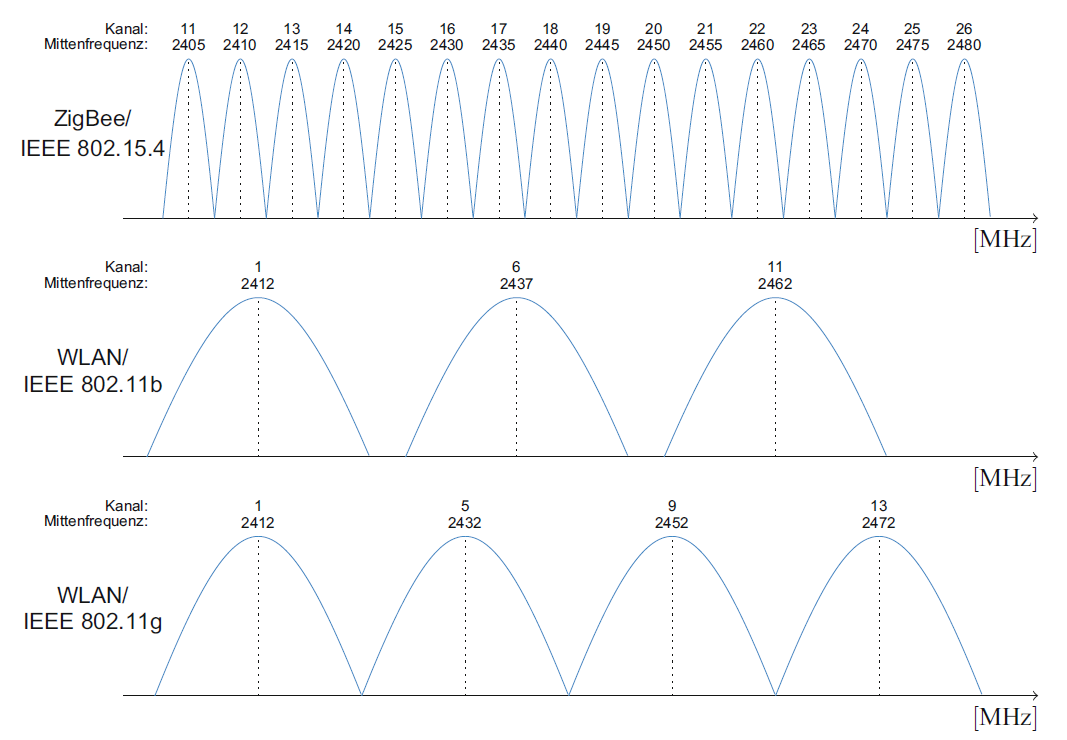
\includegraphics[width=0.8\textwidth]{Funkkanaele_Konkurrenz_IEEE.png}
	\caption{Konkurrenz IEEE und WLAN Funkkanäle \cite{markus_krause_rainer_konrad_drahtlose_2014}}
	\label{fig:KonkurrenzIEEEundWLANFunkkanäle}
\end{figure}

\subsubsection{ZCL Level Cluster}\label{subsubsec:ZCLLevelCluster}
Der Performancevergleich der Mesh Protokolle soll gemäss Benchmark Konzept (siehe Abschnitt \ref{sec:BenchmarkKonzeptMeshNetzwerke}) auf Applikationsebene durchgeführt werden.
Wie im Abschnitt \ref{Application Layer (APL)} beschrieben wird diese gebildet durch die \textit{Zigbee Cluster Library (ZCL)}.
Für den Versand von Benchmark Nachrichten wurde deshalb der \textit{ZCL Level control cluster} implementiert.
Dieser definiert Attribute und Funktionen zur Steuerung eines Gerätes welches einen Level Wert annehmen kann, wie beispielsweise die Helligkeit einer Lampe.
Die verwendete SDK stellt den \textit{ZCL Level control cluster} standardmässig zur Verfügung.\cite{the_zigbee_alliance_zigbee_2016}


\subsubsection{Enpoint Handler}\label{subsubsec:EnpointHandler}
Der Empfang von jeglichen \textit{ZCL} Nachrichten wird in der \textit{nRF5 SDK for Thread and Zigbee} durch einen Callback Handler realisiert.
Dieser wird beim Start der Anwendung einmalig registriert und ausgelöst durch ein Callback-Ereignis der Radio Schnittstelle.
Im Zigbee Benchmark wurde ein \textit{Costum Endpoint Handler} implementiert mit welchem die Benchmark Nachrichten ausgewertet werden können.
Nachrichten welche an den entsprechend Endpoint (siehe Abschnitt \ref{subsubsec:ApplicationLayer}) gesendet werden, werden in diesem Handler verarbeitet.
Die Registration des Handlers erfolgt durch den folgenden API Aufruf:

ZB\_AF\_SET\_ENDPOINT\_HANDLER(BENCHMARK\_SERVER\_ENDPOINT,\linebreak bm\_ep\_handler)

\subsubsection{APS Frame}\label{subsubsec:ZigbeeAPSFrame}
Während eines Benchmark Vorganges werden mit jeder Benchmark Nachricht die notwendigen Messgrössen gemäss Abschnitt \ref{subsec:VergleichswerteundMessgrössenMesh} generiert.
Dazu muss der \textit{Server Node}, also der Empfänger einer Nachricht, folgende Werte aus den Headern des Pakets auslesen:

\begin{itemize}
\item \textbf{Source Address:} Dies ist die Adresse in Form der \textit{Short-Address} des Senders.
\item \textbf{Message ID:} Sequenznummer der empfangenen Benchmark Nachricht.
\end{itemize}

Diese Daten können dem APS Header des Pakets, welcher in Abbildung \ref{fig:AufbauAPSDatenframe} dargestellt ist, entnommen werden.
Die Message ID wird als \textit{uint\_16t}-Wert im \textit{Manufacturer Specific} Feld des erweiterten APS Header übermittelt.
Damit können 65535 Benchmark Nachrichten eindeutig identifiziert werden.
Die eigentliche Sequenznummer des ZCL Pakets ist nur ein \textit{uint\_8t}-Wert und kann deshalb nur bis zu einem Maximalwert von 255 inkrementiert werden.
Die Identifikation der Benchmark Nachrichten wäre somit aufwendiger.

\begin{figure}[h]
	\centering
	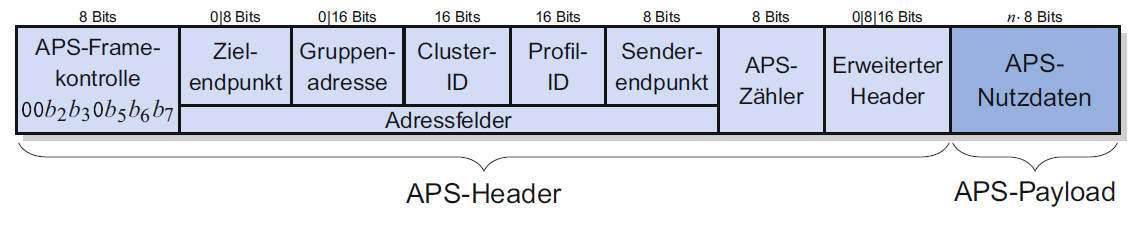
\includegraphics[width=0.8\textwidth]{Zigbee_APS_Datenframe.png}
	\caption{Aufbau APS Datenframe \cite{markus_krause_rainer_konrad_drahtlose_2014}}
	\label{fig:AufbauAPSDatenframe}
\end{figure}


\subsubsection{Adressierung}\label{subsubsec:Adressierung}
Die Adressierung der Nodes innerhalb des Zigbee Mesh Benchmarks kann entweder Unicast oder Multicast erfolgen.
Eine Multicast Adressierung kann mit Hilfe des \textit{ZCL Groups cluster} erfolgen.
Dazu wird der Cluster auf den entsprechenden Nodes implementiert und diese werden mittels \textit{ZCL Add Group Request}-Befehl einer gewissen Gruppe hinzugefügt.
Eine solche Adressierung kann gemäss Abschnitt \ref{subsubsec:CLI} durch die Angabe einer \textit{Group Number} in der Konfiguration der Benchmark Nodes definiert werden.
Funktionstests zu Beginn der Benchmark Messungen haben allerdings gezeigt, dass diese Multicast Adressierung auf diesem Wege nicht praktikabel ist (siehe Abschnitt \ref{subsubsec:Group addressing mode}).
Deshalb wurden die Zigbee Benchmark Messungen im Unicast Modus durchgeführt.
Dabei werden die Benchmark Nachrichten direkt an die jeweiligen Empfänger gesendet.
Die Unicast Adressierung erfolgt durch Angabe der MAC Adressen der Empfänger bei der Konfiguration der Client Nodes.
Durch Abfrage der \textit{Adress-Table} werden schliesslich die \textit{Short-Addresses} der Empfänger ermittelt.


\subsection{Mesh Node Firmware}\label{subsec:ZigbeeMeshNodeFirmware}
Die Firmware für die Benchmark Nodes die in Abschnitt \ref{sec:Soft-undFirmware} bereits behandelt wurde, wird durch ein C- und ein H-Modul ergänzt die spezifisch für die Implementation des Zigbee Stack zuständig sind.
Im Modul \textit{bm\_config.h} werden Konstanten für den Benchmark wie auch die Funktion des Stacks definiert.
Das Modul \textit{bm\_zigbee.c} hingegen beinhaltet je nach Funktion des Nodes (Master, Client oder Server) die entsprechenden Funktionen für die Initialisierung und Konfiguration des Stacks sowie das Benchmark Handling.
Darin ist der Versand und Empfang der Benchmark Nachrichten vereint.
Der gesamte Sourcecode ist im Github Repository\footnote{\url{https://github.com/Rouben94/P6_Software} \cite{anklin_bobst_horath_rouben94p6_software_nodate}} zu diesem Projekt einsehbar.

\subsubsection{Stack Init und Konfiguration}\label{subsubsec:ZigbeeStackInitundKonfiguration}
Die Stack Init Routine wird durch die Benchmark Statemachine gemäss Abschnitt \ref{subsubsec:StatemachineSoftware} im State \textit{Init Benchmark} aufgerufen.
Diese Routine ist durch die Funktionen \textit{bm\_zigbee\_init()} sowie \textit{bm\_zigbee\_enable()} im Modul \textit{bm\_zigbee.c} abgebildet.
Hier wird der Zigbee Stack in der Rolle als \textit{Zigbee-Koordinator} resp. \textit{Zigbee-Server} initialisiert und hochgefahren.

Nach dem Start des Stacks wird der \textit{ZBOSS Mainloop} im Benchmark State iteriert. Damit wird der \textit{ZBOSS Scheduler} aktiviert und die Ausführung des Stacks startet.

Der \textit{Zigbee-Koordinator} welcher auf dem Benchmark Master Node aufgesetzt ist, startet nun das \textit{Network Formation}, sofern keine Konfiguration gespeichert ist.
Dies ist nur beim Erststart der Fall.
Im \textit{Network Formation} wird das Zigbee Netzwerk auf dem gewählten Kanal gebildet und die entsprechenden Netzwerk Schlüssel generiert.
Kann beim Start eine Konfiguration aus dem Flash gelesen werden oder das \textit{Network Formation} war erfolgreich, wird direkt mit dem \textit{Zigbee Commissioning} gestartet.

Im \textit{Zigbee Commissioning} State melden sich sämtliche Teilnehmer beim \textit{Zigbee-Koordinator} an und erhalten von ihm die nötigen Netzwerkparameter.
Unter anderem wird jedem Node eine 16-Bit \textit{Short-Address} zugewiesen.
Der Start des \textit{Commissioning} wird bei den Benchmark Teilnehmern um eine zufällige Zeit zwischen 0 und 30 Sekunden verzögert.
So kann sichergestellt werden, dass der \textit{Zigbee-Koordinator} nicht von Anfragen überhäuft wird.
Nach erfolgreichem \textit{Commissioning} ist das Zigbee Mesh Netzwerk bereit für die erste Messung.

Die gesamte \textit{Benchmark Init} Phase wie sie im Abschnitt \ref{subsubsec:StatemachineSoftware} definiert wurde dauert bei Zigbee 60 Sekunden.
Diese Zeit wird benötigt um das \textit{Commissioning} abzuschliessen.
Danach wird automatisch in den \textit{Benchmark State} gewechselt.

\subsubsection{Benchmark Handling}\label{subsubsec:ZigbeeBenchmarkHandling}
Während der Master am Benchmark Handling nicht beteiligt ist,  sind im Modul \textit{bm\_zigbee.c} für den Benchmark Client und den Benchmark Server unterschiedliche Funktionen implementiert.

\paragraph{Client}
Der Benchmark Client ist für den Versand von Benchmark Nachrichten zuständig.
Dazu wird durch die Benchmark Statemachine mittels universeller Schnittstelle in der SharedLib (siehe Abschnitt \ref{subsec:SharedLibrary} die Funktion \textit{bm\_send\_message()} aufgerufen.
Diese löst wiederum einen Callback aus in welchem die Benchmark Nachricht konstruiert und schliesslich versendet wird.
Die Nachricht ist einem \textit{ZCL Move to Level Request} nachempfunden.
Allerdings kann die Payload der Nachricht beliebig erhöht werden.

Noch vor dem Versand der Benchmark Nachricht werden die Message Infos in der Funktion \textit{bm\_read\_message\_info()} ausgelesen und ein Log-Eintrag wird erstellt.
Dabei handelt es sich um die Messgrössen gemäss Abschnitt \ref{subsec:VergleichswerteundMessgrössenMesh}.
Zudem wird der Zustand des grünen RGB-LEDs gewechselt.

\paragraph{Server}
Der Benchmark Server wartet im \textit{Benhmark State} auf ankommende Benchmark Nachrichten.
Sobald ein Paket vom Stack empfangen wurde, wird der Benchmark Endpoint Handler\linebreak \textit{(bm\_ep\_handler())} signalisiert.
Dieser entscheidet anhand der \textit{ZCL Cluster ID} ob es sich bei der Nachricht um eine Benchmark Nachricht handelt.
Falls dem so ist, wird die Funktion \textit{bm\_receive\_message()} aufgerufen und die Referenz des Paket Buffers \textit{(bufid)} übergeben.
Mit Hilfe der \textit{bufid} werden nun die Message Infos ausgelesen und daraus ein Log Eintrag erstellt.
Zum Schluss wird der Status des blauen RGB-LED's gewechselt womit der erfolgreiche Empfang einer Nachricht signalisiert wird.




\subsubsection{Benchmark und Stack Parameter}\label{subsubsec:BenchmarkundStackParameter}
Für die Umsetzung des Zigbee Protokoll Stacks sowie des Benchmark Frameworks für den Zigbee Benchmark, mussten einige Parameter gesetzt oder neu definiert werden.
Die Tabelle \ref{tab:ZigbeeBenchmarkundStackParameter} zeigt die wichtigsten Benchmark und Stack Parameter.

\begin{table}[h]
\centering
\begin{adjustbox}{width=1\textwidth}
\begin{tabular}{lll}
Stack Init Time & 60000 ms & \begin{tabular}[t]{@{}l@{}}Zeit die benötigt wird um den Stack für den Benchmark\\zu initialisieren. Das Zigbee Netzwerk benötigt eine\\gewisse Zeit um sich aufzubauen \end{tabular} \\
STACK\_STARTUP\_MAX\_DELAY & 30000 ms & \begin{tabular}[t]{@{}l@{}}Maximalwert für die Verzögerungszeit des Stack Startup\\bei Client und Server Nodes.\end{tabular} \\
NETWORK\_FORMATION\_DELAY & 5000 ms & \begin{tabular}[t]{@{}l@{}}Verzögerungszeit für das Network Formation durch \\den Koordinator. \end{tabular} \\
IEEE Channel & 15 & Zigbee Kanal der verwendet wird um das Mesh aufzubauen. \\
Client Endpoint & 1 & Nummer für den Client Endpoint im ZCL Level Cluster \\
Server Endpoint & 10 & Nummer für den Server Endpoint im ZCL Level Cluster \\
Group ID & 0xB331 & \begin{tabular}[c]{@{}l@{}}Default Group ID. Zu diesem Wert wird der Index für die\\zugewiesene Gruppe addiert um die\\Gruppenzugehörigkeit festzulegen.\end{tabular}
\end{tabular}
\end{adjustbox}
\caption{Zigbee Benchmark und Stack Parameter}
\label{tab:ZigbeeBenchmarkundStackParameter}
\end{table}